\documentclass[a4paper]{article}    % base article class
\usepackage[utf8]{inputenc}         % allow utf8 input
\usepackage{textalpha}              % enable greek utf8 in text
\usepackage{alphabeta}              % enable greek utf8 in math
\usepackage{graphicx}               % includegraphics
\usepackage{amsmath,amsthm}         % fancier math
%
%\usepackage{ebgaramond}
%
%\usepackage{newtxtext}               % times new roman font
%\usepackage[bigdelims,cmintegrals,vvarbb]{newtxmath}
%
\usepackage[osf,sups]{Baskervaldx} % lining figures
\usepackage[bigdelims,cmintegrals,vvarbb,baskervaldx,frenchmath,upint]{newtxmath} % math font
%\usepackage{cabin}                  % monospace font
\usepackage[cal=boondoxo]{mathalfa} % mathcal from STIX, unslanted a bit
%
\usepackage{hyperref,url}           % hyperlinks and urls
\usepackage{fancyvrb}               % fancier verbatim environment
\usepackage[x11names]{xcolor}                 % for colors
%\usepackage{pdflscape}              % for landscape pages
%\delimitershortfall-1sp
%\usepackage{mleftright}              % enlarge nested parentheses
%\mleftright
\setlength{\parindent}{0pt}         % no paragraph indentation
\setlength{\parskip}{7pt}           % spacing between paragraphs
\setlength{\emergencystretch}{3em}  % prevent overfull lines
\pdfimageresolution 200             % change the default for included png files
\pdfinfoomitdate=1\pdftrailerid{}   % ensure reproducible PDF
\makeatletter\renewcommand{\verbatim@font}{\ttfamily\footnotesize}\makeatother
\newenvironment{gallery}{}{}
\newcommand{\galleryline}[1]{\includegraphics{#1}{\footnotesize\tt #1}\newline}
\theoremstyle{note}
\newtheorem{exercice}{Exercice}
\swapnumbers
\theoremstyle{plain}
\newtheorem{theorem}{Theorem}[section]
\newtheorem{lemma}[theorem]{Lemma}
\newtheorem{remark}[theorem]{Remark}
\newtheorem{definition}[theorem]{Definition}
\newtheorem{proposition}[theorem]{Proposition}

\begin{document}

\title{tropomi pixel gain correction}
\date{}
\maketitle


\section{Introduction}

If you work with TROPOMI products you'll certainly recognize these
characteristic diagonal streaks

\begin{tabular}{ll}
	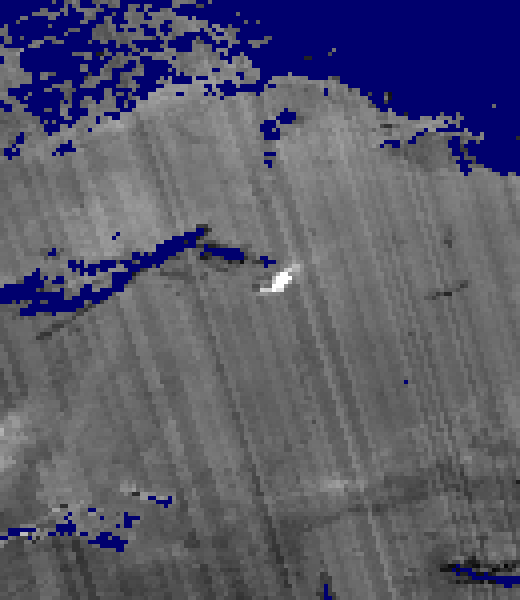
\includegraphics[width=.4\textwidth]{f/kccplume20b.png} &
	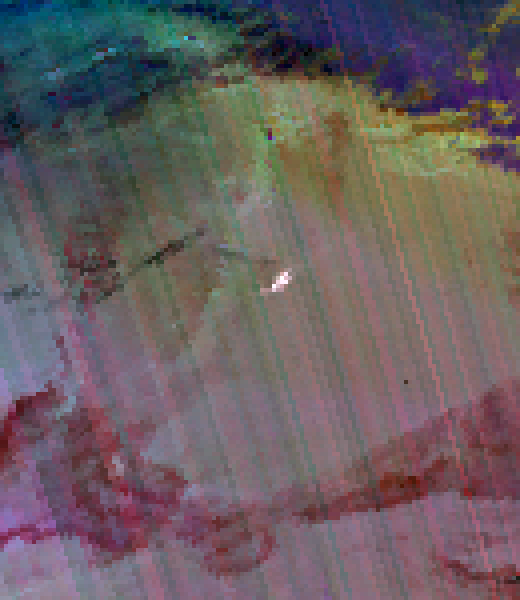
\includegraphics[width=.4\textwidth]{f/ikniceshot.png} \\
%	L2 product & Heuristic from L1
\end{tabular}

These streaks only seem to be diagonal because you are resampling the image on a
(longitude, latitude) grid.  In the raw image, which is acquired from a
slightly oblique orbit, they are aligned with the pixel grid


% plambda TRANS[flip=topdown,y=880,h=240]:S5P_OFFL_L2__CH4____20200105T112716_20200105T130846_11550_01_010302_20200107T042409.nc,methane_mixing_ratio_bias_corrected  'x 1e30 > nan x if'|qeasy 1830 1940|plambda 'x x 0 0 110 rgb if'|homwarp -o 0 -i "2 0 0 0 1 0 0 0 1" 430 240 |ntiply 4 - ~/cropblue.png
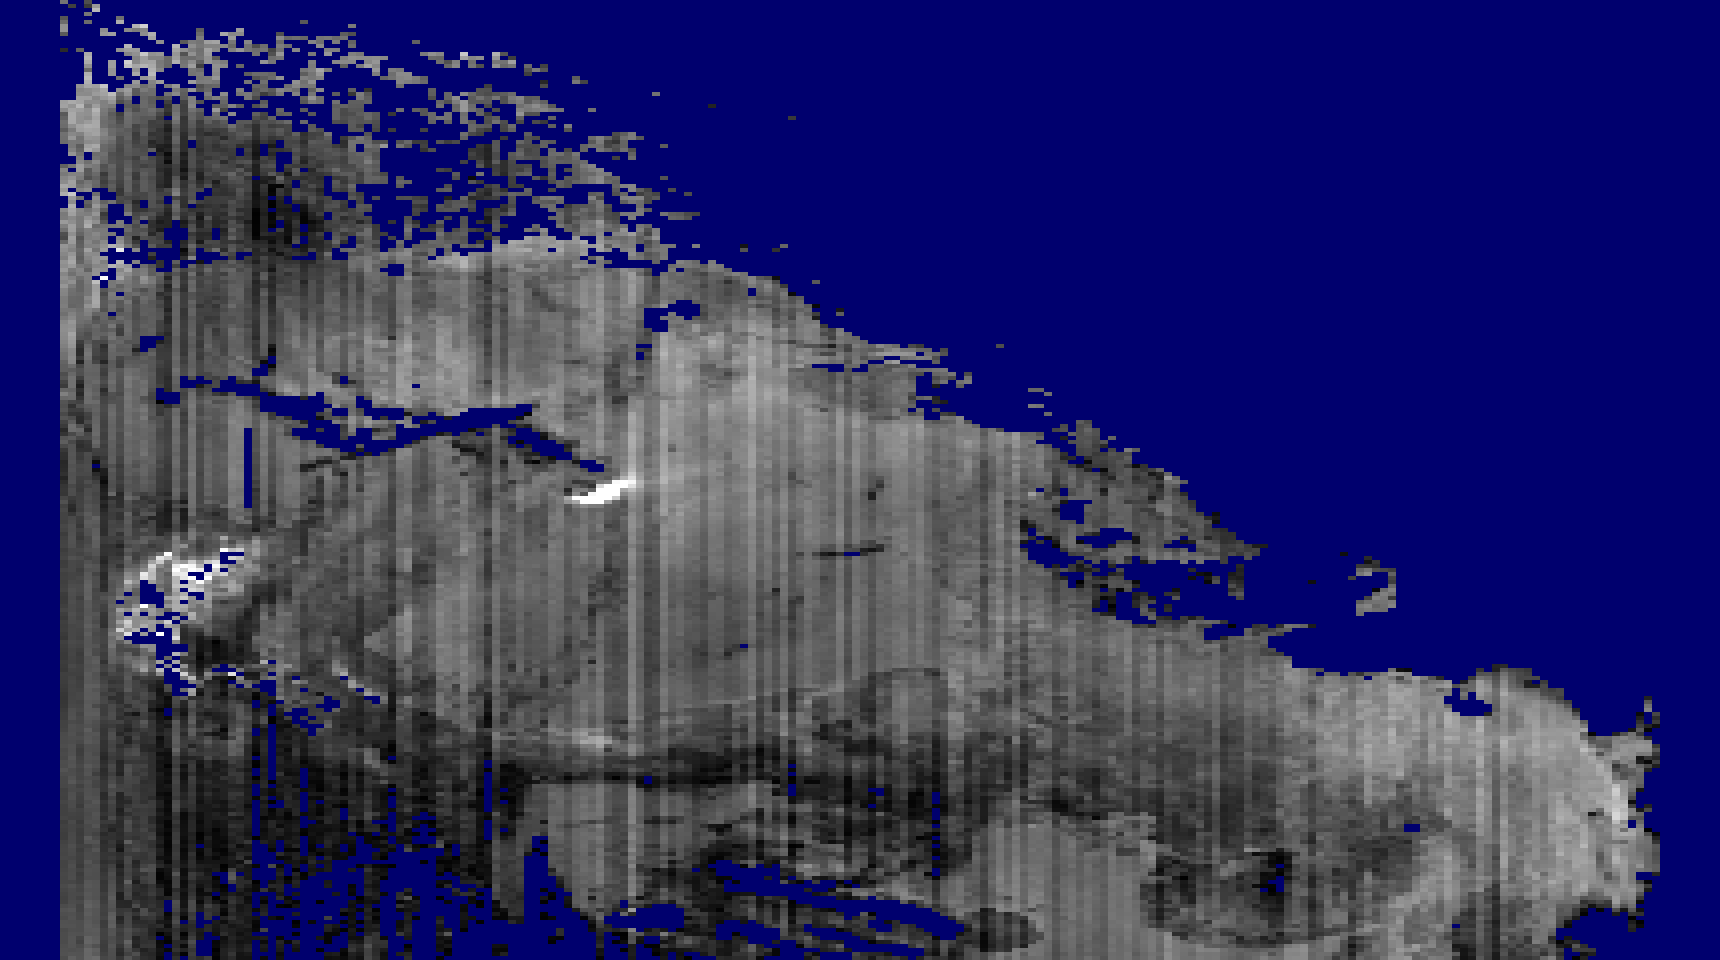
\includegraphics[width=.8\textwidth]{f/cropblue.png}

The objective of this note is to understand the origin of these artifacts and
propose two methods to remove them.

\section{Formation of the artifacts in the sensor}

The TROPOMI instruments contains four spectrometers: UV, UVIS, NIR and SWIR.
For archival purposes, the data of each of the detectors is divided in two
halves, which yields a total of eight spectral bands.  The UV, UVIS and NIR
detectors are three identical CCD matrices of size~$1024\times 1024$, of
which only about~$864$ rows are illuminated by the signal.  The SWIR detector
is a MCT ROIC matrix of size~$1000\times 256$.

The following images show (in normalized logarithmic scale) the input of each
of the four detectors at the moment the satellite view the sun glint, which
is visible as the bright horizontal line, especially on the UVIS and NIR
detectors.  The horizontal lines in the images correspond to the rest of
geographical features, with the sea begin the two dark bands at the bottom of
the sensor and around the glint.  The curved almost vertical features are the
absorption lines on the spectrum due to the earth and sun atmospheres, the
most prominent one being the~$O_2$ band near the left of the NIR image.

\begin{tabular}{ll}
	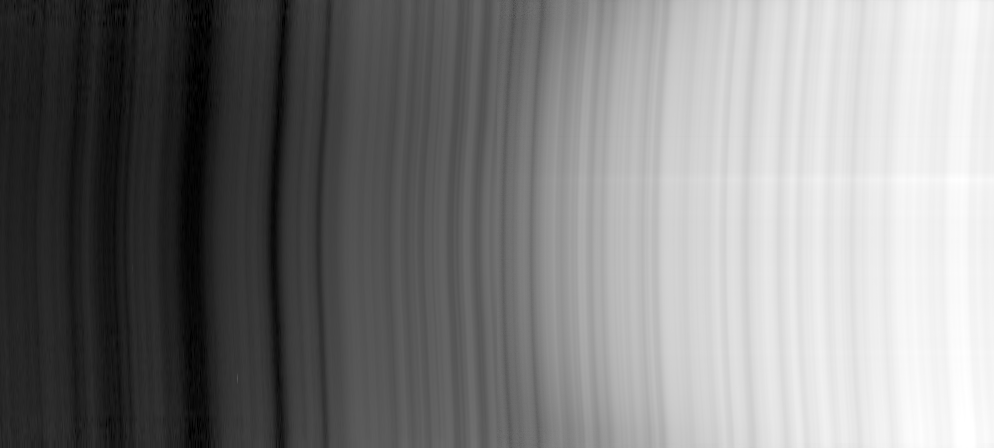
\includegraphics[width=0.48\linewidth]{f/lglint_12.png} &
	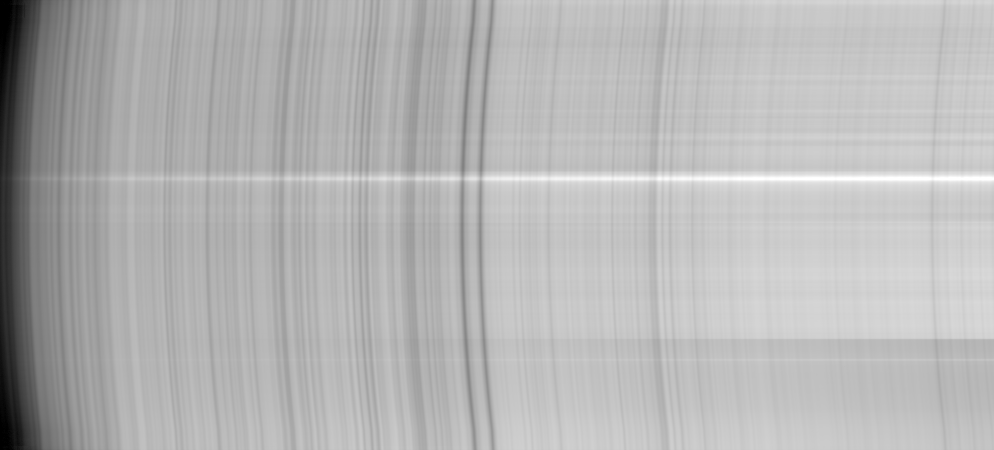
\includegraphics[width=0.48\linewidth]{f/lglint_34.png} \\
	UV (bands 1 and 2)& UVIS (bands 3 and 4) \\
	& \\
	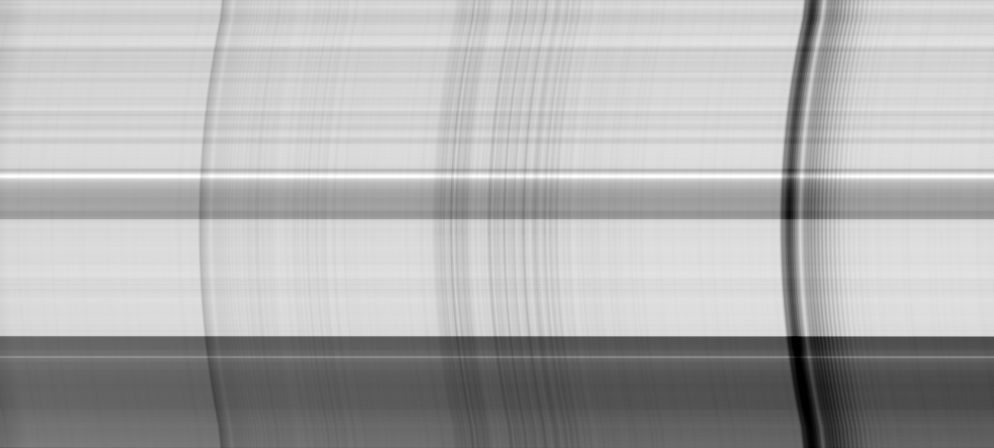
\includegraphics[width=0.48\linewidth]{f/lglint_56.png} &
	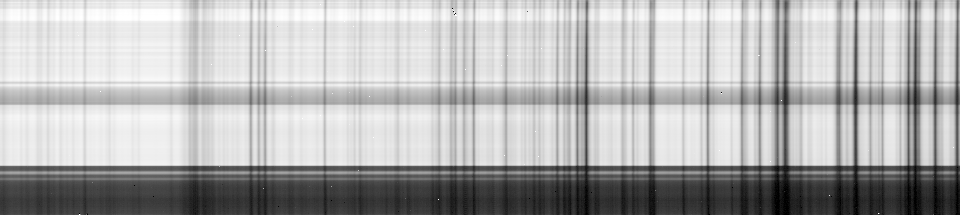
\includegraphics[width=0.48\linewidth]{f/lglint_78.png} \\
	NIR (bands 5 and 6) & SWIR (bands 7 and 8)
\end{tabular}

To better understand the geometry of the acquisition, we can compute the
average of all the spectral samples on band 4 (visible), along a half-orbit.
This is the resulting image, notice the glint at the southernmost tip of the
Mediterranean sea.

\begin{tabular}{l}
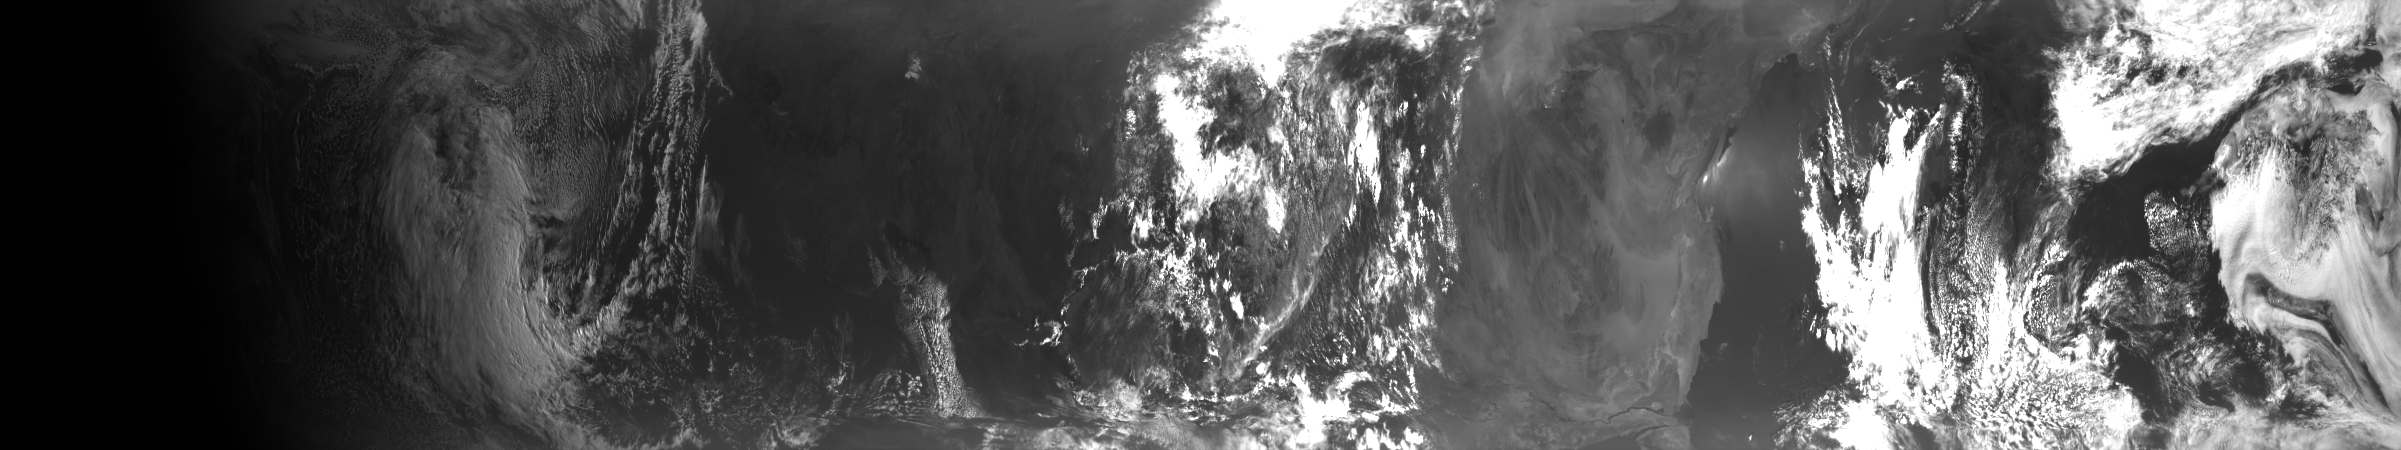
\includegraphics[width=\linewidth]{f/rslice_b4_glint.png} \\
Average of all channels on band 4 (north to the right)
\end{tabular}

So far, nothing seems obviously wrong in these images.  But there are two
problems in these images that become apparent when we look at them closely.
The two sources of anomalous readings are: (1) biases in the gain of each
pixel, which are not constant but vary slowly in time and (2) transient
pixels due to cosmic rays hitting the sensor array.  The gain of each pixel
is typically correlated along columns of the array, giving a characteristic
texture similar to that of the infrared cameras, that can be corrected by
standard means.  The transient pixels are isolated in space and frequency and
can be removed due to the local smoothness of the data.

The disparities in pixel gain become apparent when we compute the average
of captor acquisitions along track.  We start with band 6 which is slightly
easier to understand.  This is the average captor input on band 6 along a
half-orbit, and a detail of its Laplacian:

\begin{tabular}{ll}
	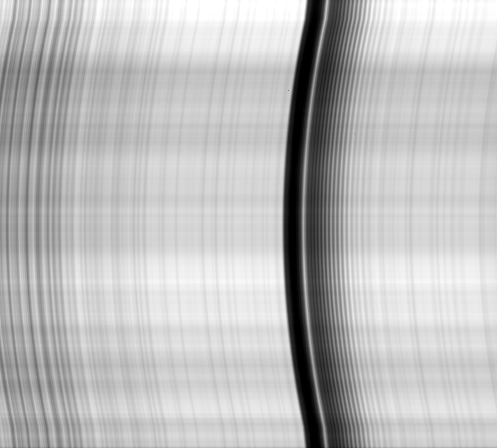
\includegraphics[width=0.5\linewidth]{f/b6_avgs.png} &
	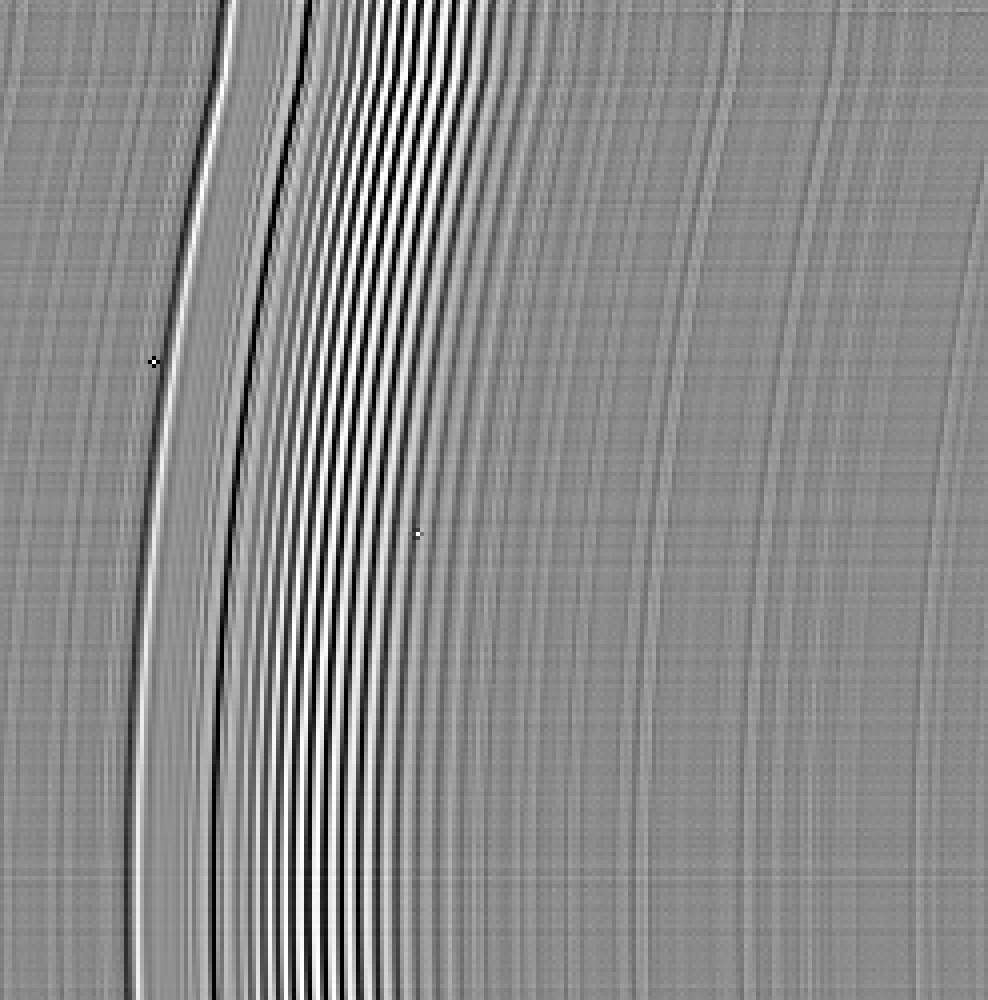
\includegraphics[width=0.5\linewidth]{f/b6_lapavgs.png} \\
	$\mathrm{avg}$ & $\Delta\mathrm{avg}\qquad$ (detail, upper-right corner)
\end{tabular}

Notice that the Laplacian enhances the location of two ``bad'' pixels.

A similar visualization for the other bands:

\begin{tabular}{llll}
	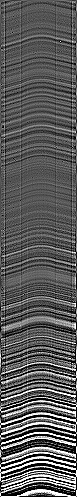
\includegraphics[height=0.38\linewidth]{f/b1_lapavgs.png} &
	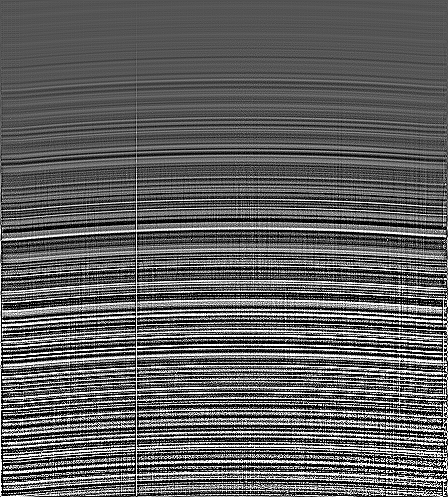
\includegraphics[height=0.38\linewidth]{f/b2_lapavgs.png} &
	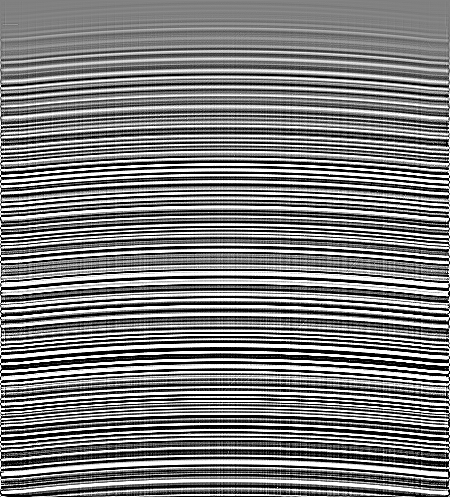
\includegraphics[height=0.38\linewidth]{f/b3_lapavgs.png} &
	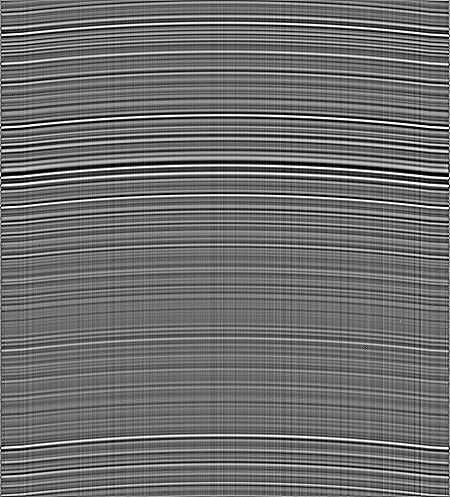
\includegraphics[height=0.38\linewidth]{f/b4_lapavgs.png} \\
	$B1$ & $B2$ & $B3$ & $B4$
\end{tabular}

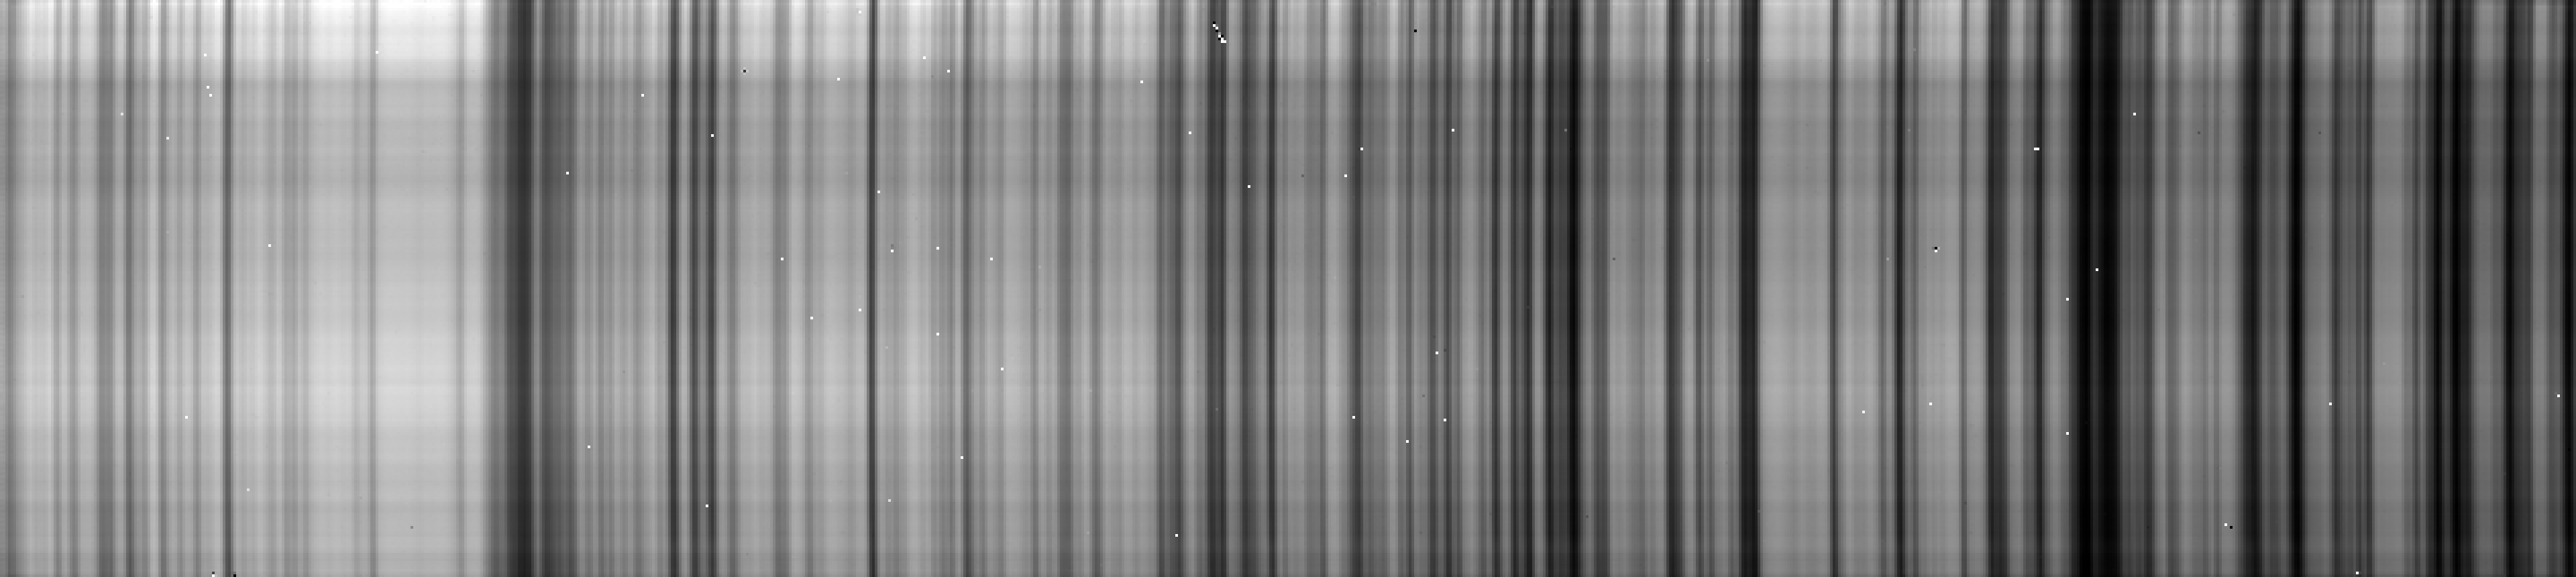
\includegraphics[width=\linewidth]{f/b78_avgs.png}%
$SWIR$

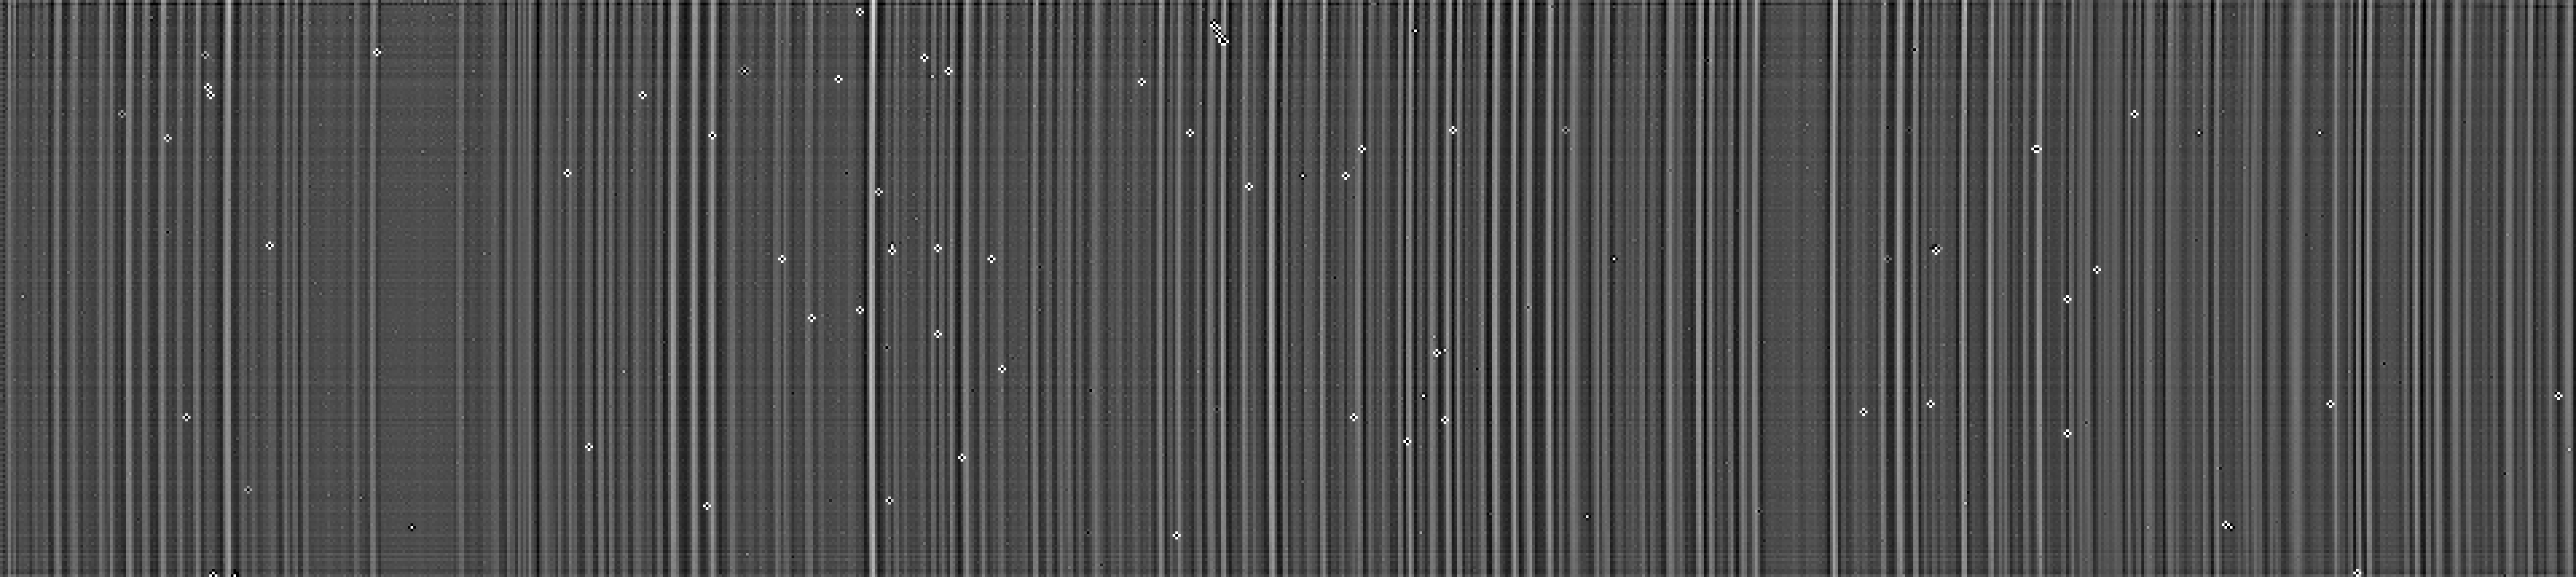
\includegraphics[width=\linewidth]{f/b78_lapavgs.png}%
$\Delta SWIR$

For the SWIR band the main problem seems to be that the gain of some individual
pixels is way off.  For the UV and visible bands, the main problem seems to
be the across-smile texture (that cannot be explained by the image contents),
as well as a few bad pixels.

The following image shows the effect of the ``bad pixel'' on band 6 when
slicing the datacube at the frequency index of that pixel:

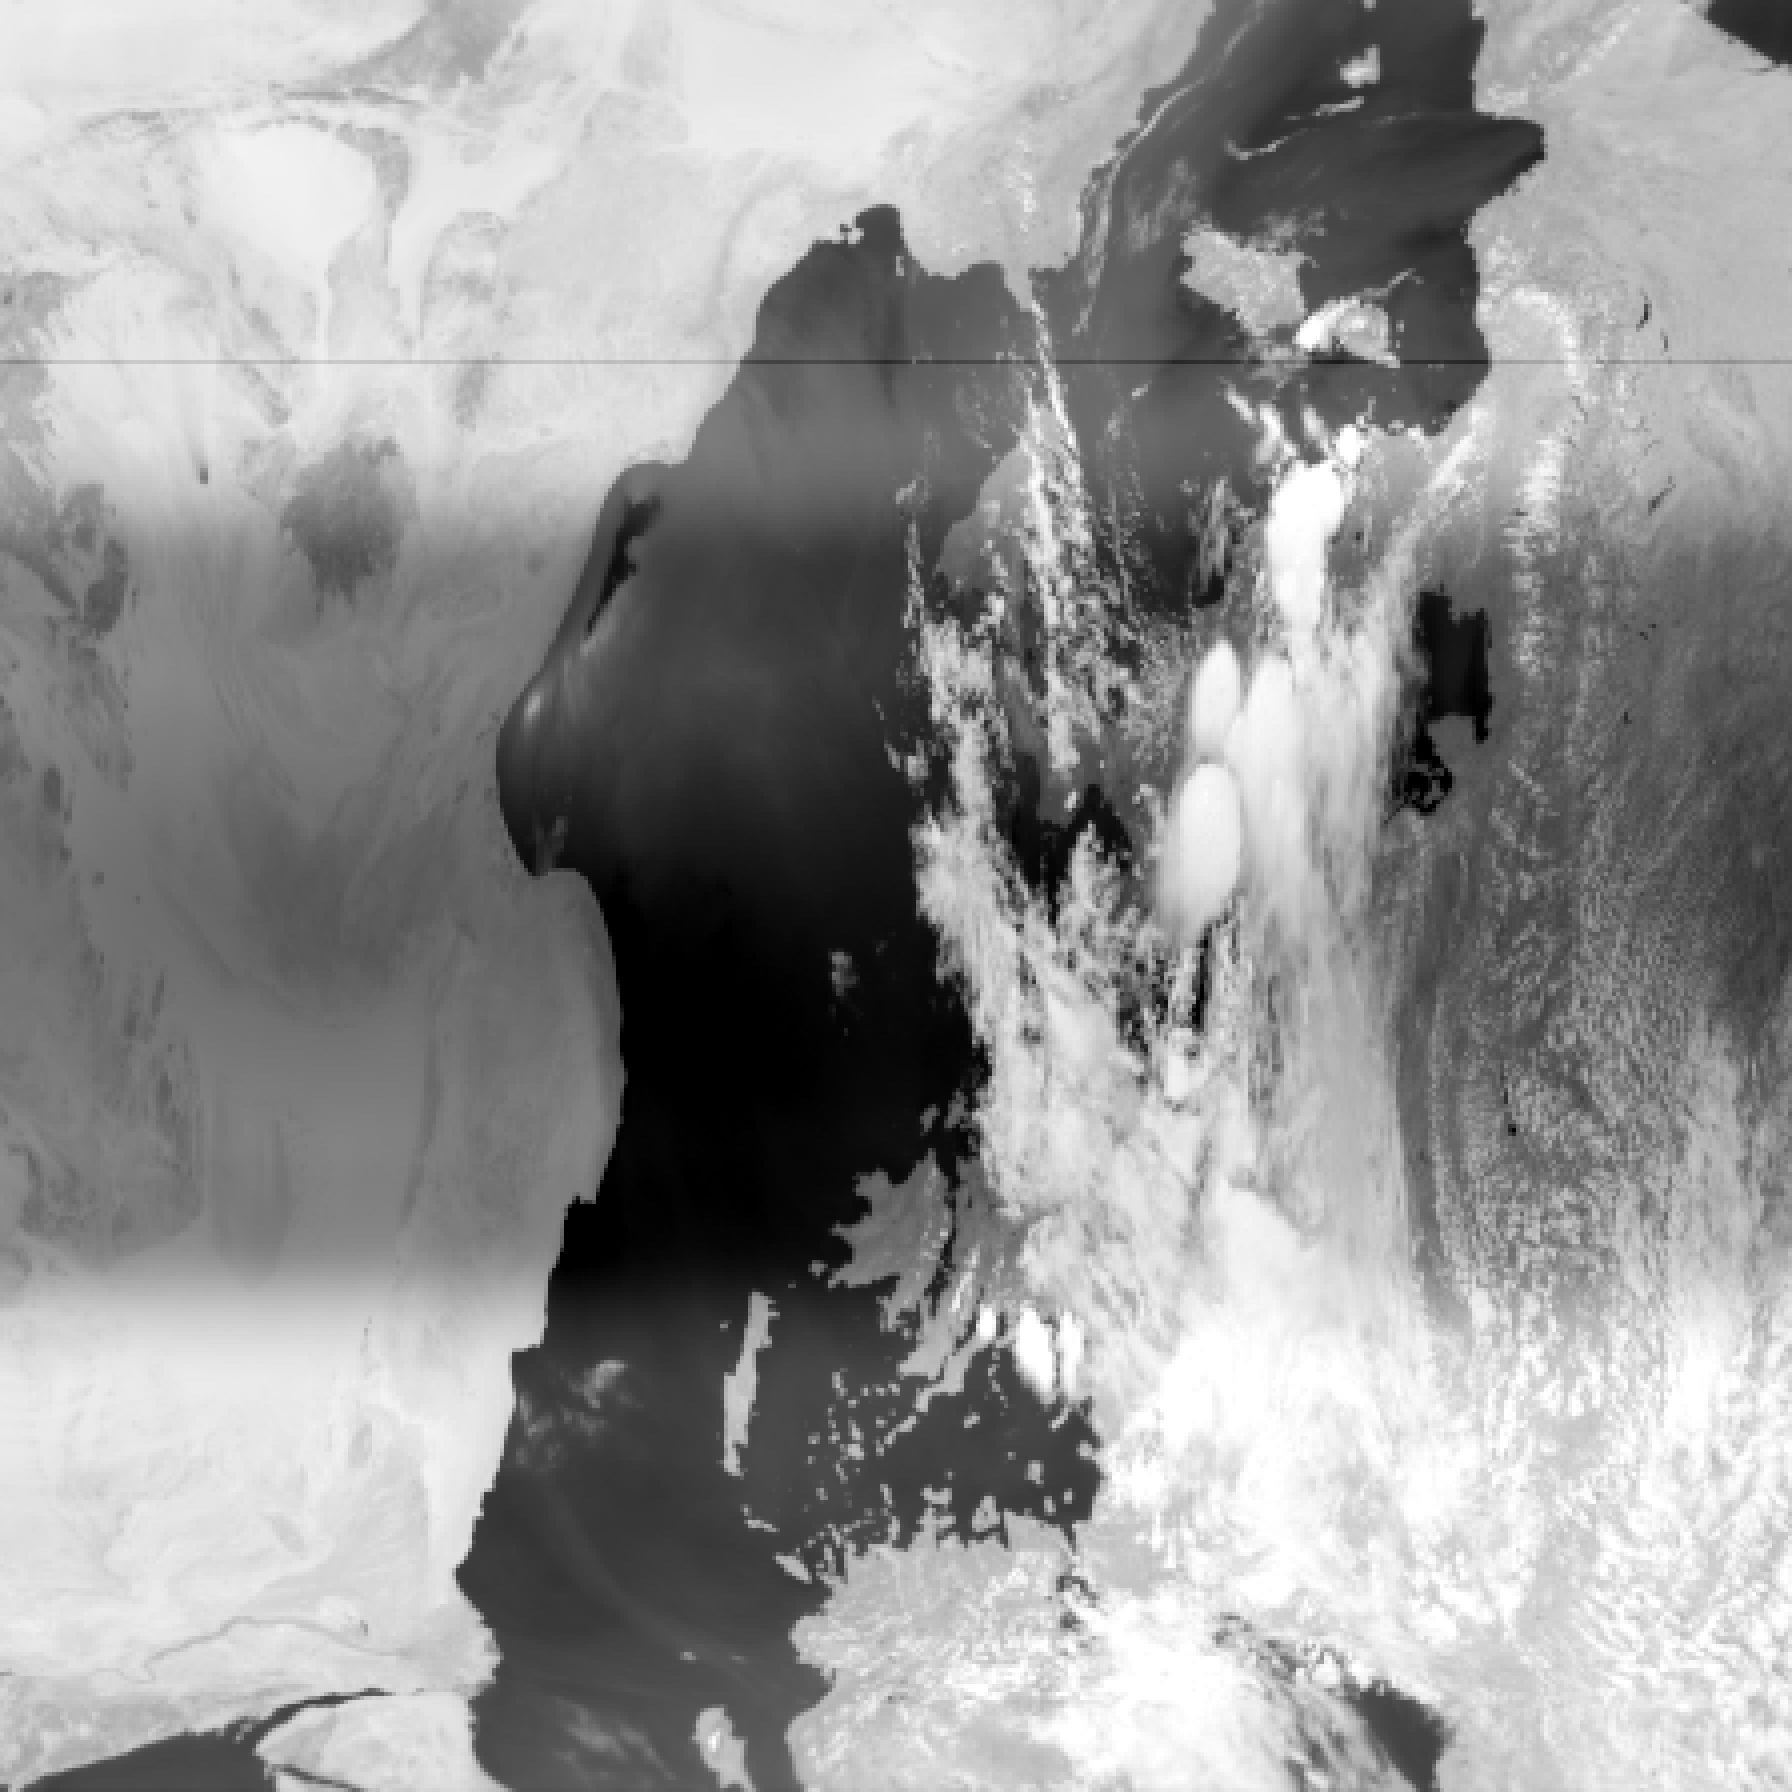
\includegraphics[width=0.8\linewidth]{f/r6_288_log.png}

The bad pixel is the darker thin line that crosses through the north of
Corsica.  The thick horizontal darker band through the middle-third of the
image is part of the~$O_2$ absorption band.

We propose two methods to correct these artifacts.

\clearpage
\section{Method 1: data-based correction}

The first method to correct the artifacts is based on a single TROPOMI image,
and using only the radiance measurements.  The algorithm is the following

1. Compute the average sensor signal over the whole datacube.  The result is
an image~$A$ of the same size as the sensor matrix.

2. Identify points where~$\Delta A$ is abnormally high or low (by setting a
hard threshold on the Laplacian, different for each band).  These are the
``bad pixels'' that result on very visible streaks further down the
processing chain.

3. At the site of each pixels location, scale all the data values along the
track (latitude) to minimize the difference between that site and the
four neighboring ones in the (wavelength/longitude) plane.  There are several
minimization criteria, the simplest one being least squares: in that case the
scaling factor is simply the value of the Laplacian at that location.

The result of this correction is shown here, to be compared to the previous
image:

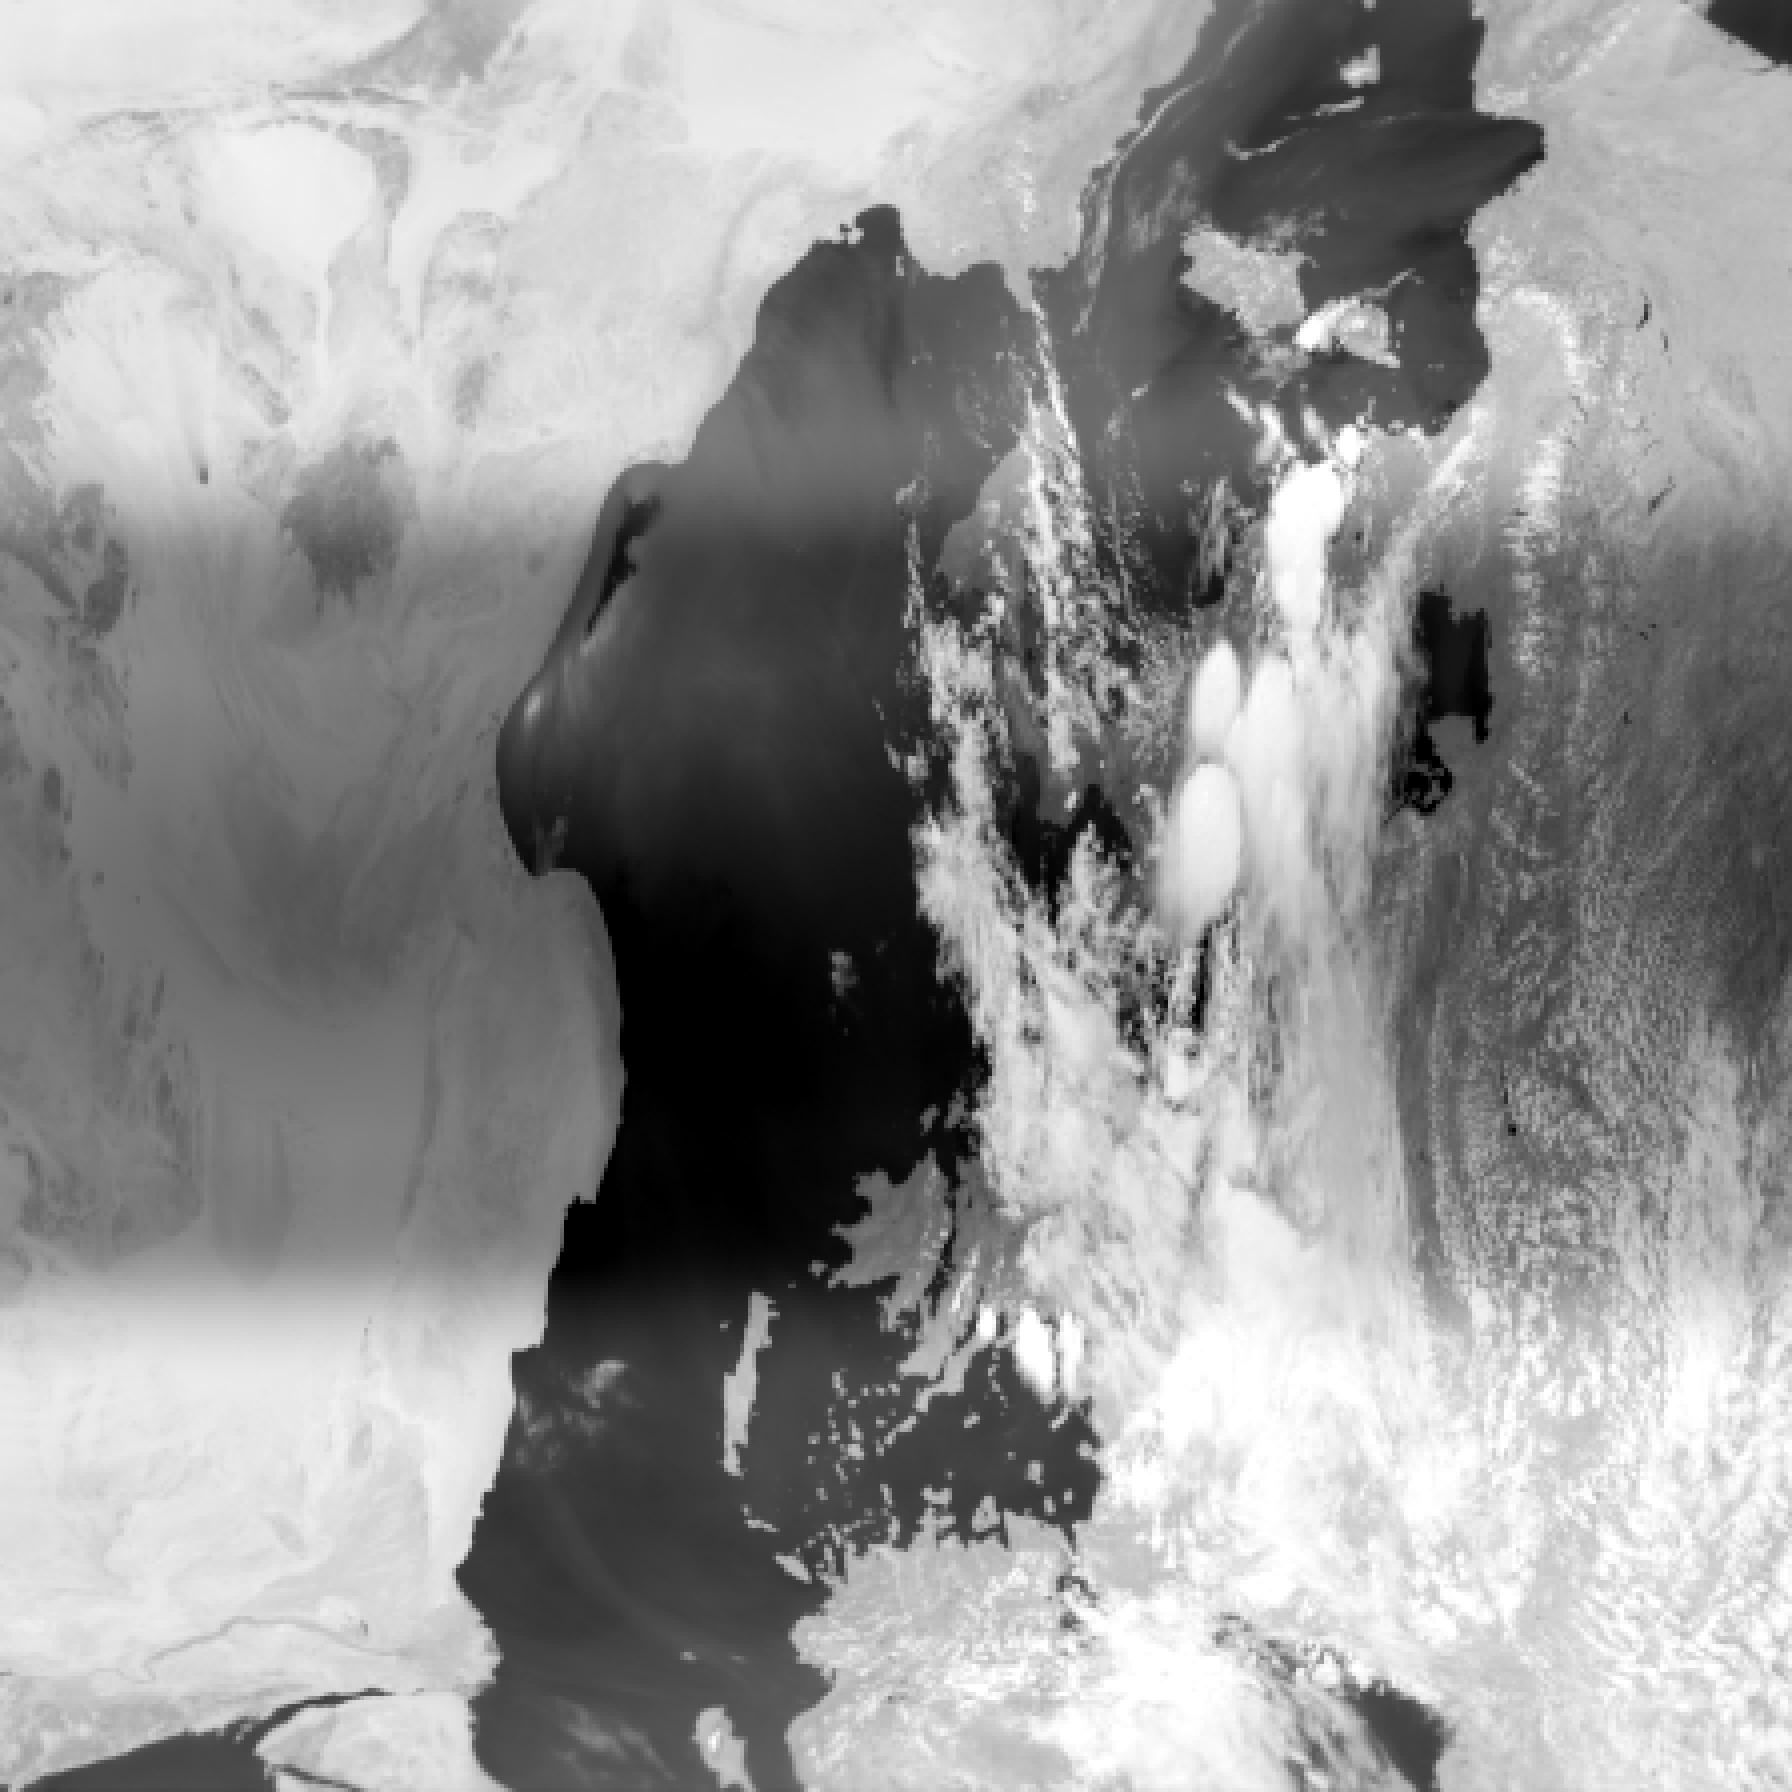
\includegraphics[width=0.8\linewidth]{f/corrected_r6_288_log.png}

This method is particularly useful in the SWIR bands, where there are many
such bad pixels.  Notice that the structured noise that is formed by
across-smile lines (and not by isolated bad pixels) is not corrected by this
method.

\clearpage
\section{Method 2: irradiance-based correction}

The second method to correct the artifacts is based on the provided TROPOMI
irradiance data, which is collected once every 15 orbits (once per day).
This data is obtained by letting unfocused sunlight reach the captor
directly.  The irradiance data is a single image of the whole sensor array
that looks like this:

\begin{tabular}{ll}
	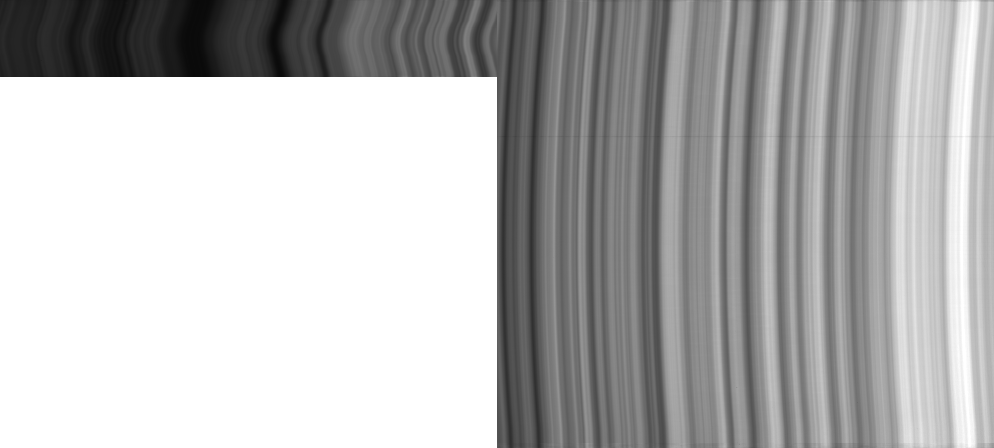
\includegraphics[width=0.48\linewidth]{f/irradiance_12.png} &
	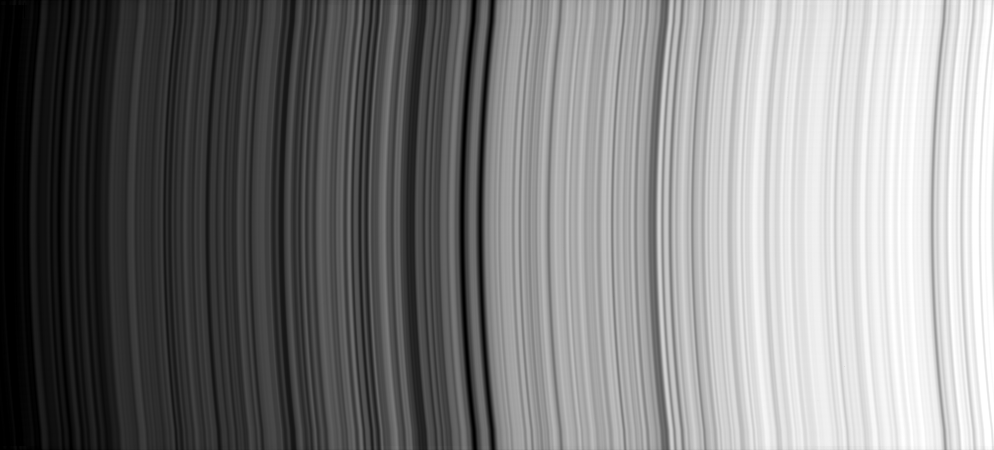
\includegraphics[width=0.48\linewidth]{f/irradiance_34.png} \\
	UV (bands 1 and 2)& UVIS (bands 3 and 4) \\
	& \\
	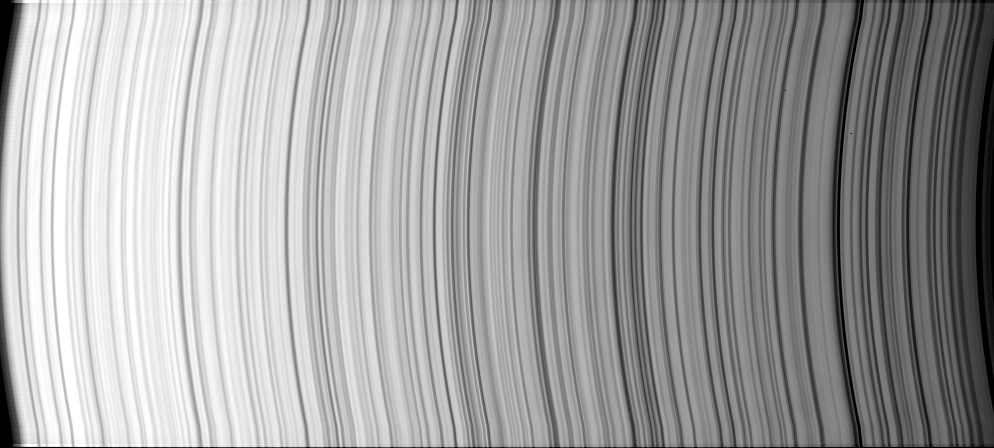
\includegraphics[width=0.48\linewidth]{f/irradiance_56.png} &
	%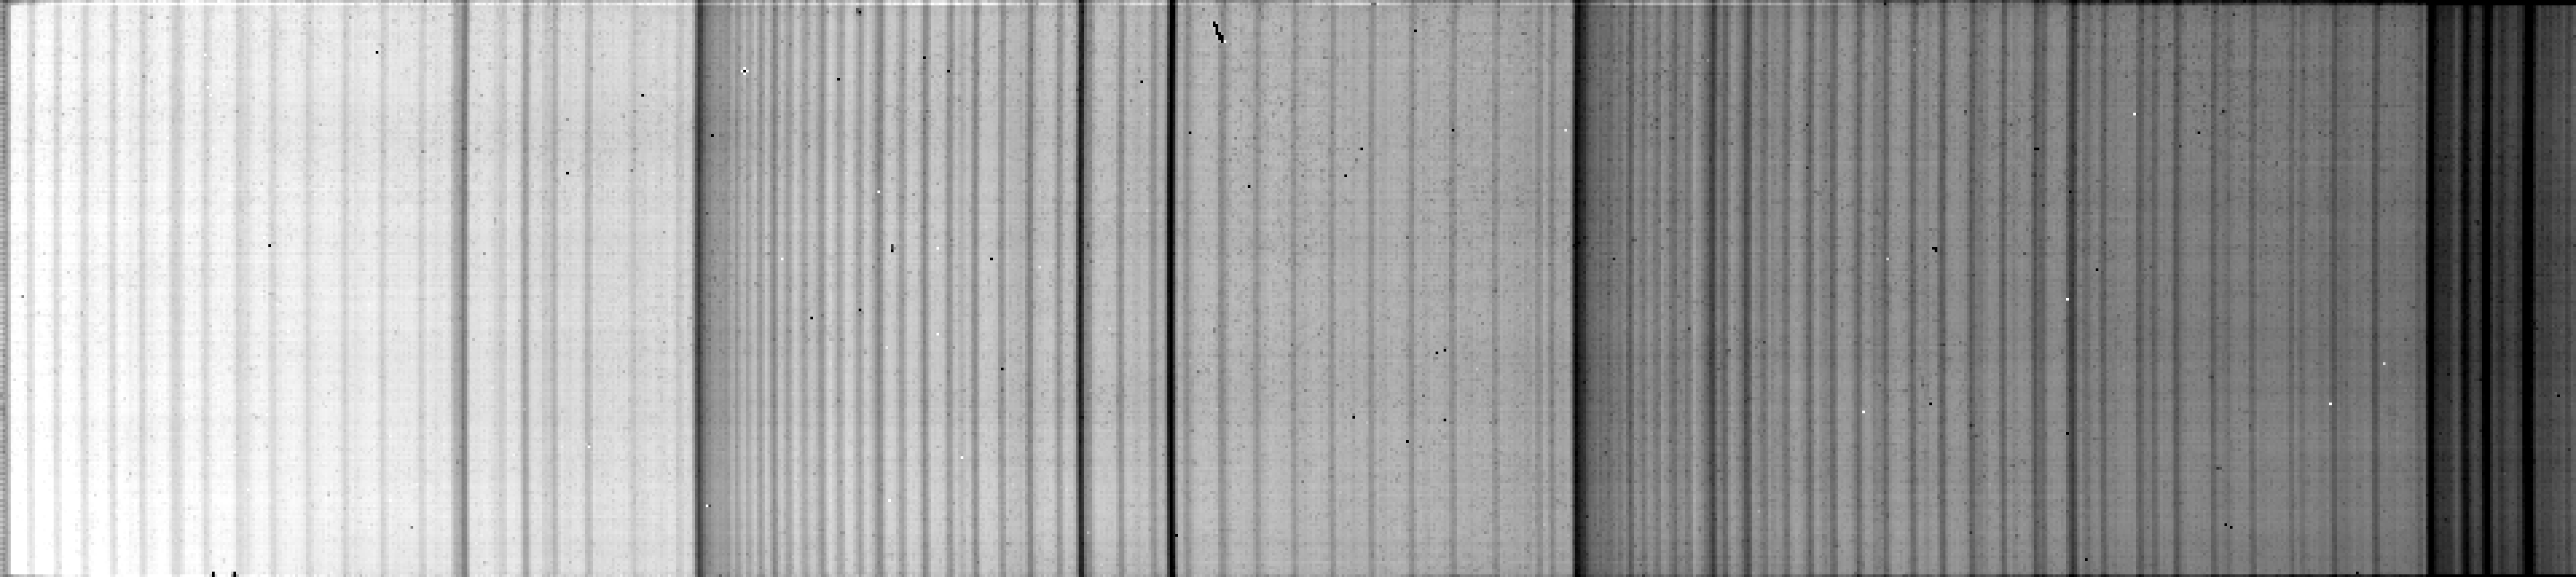
\includegraphics[width=0.48\linewidth]{f/irradiance_78.png}
	\\
	NIR (bands 5 and 6) %& SWIR (bands 7 and 8)
\end{tabular}


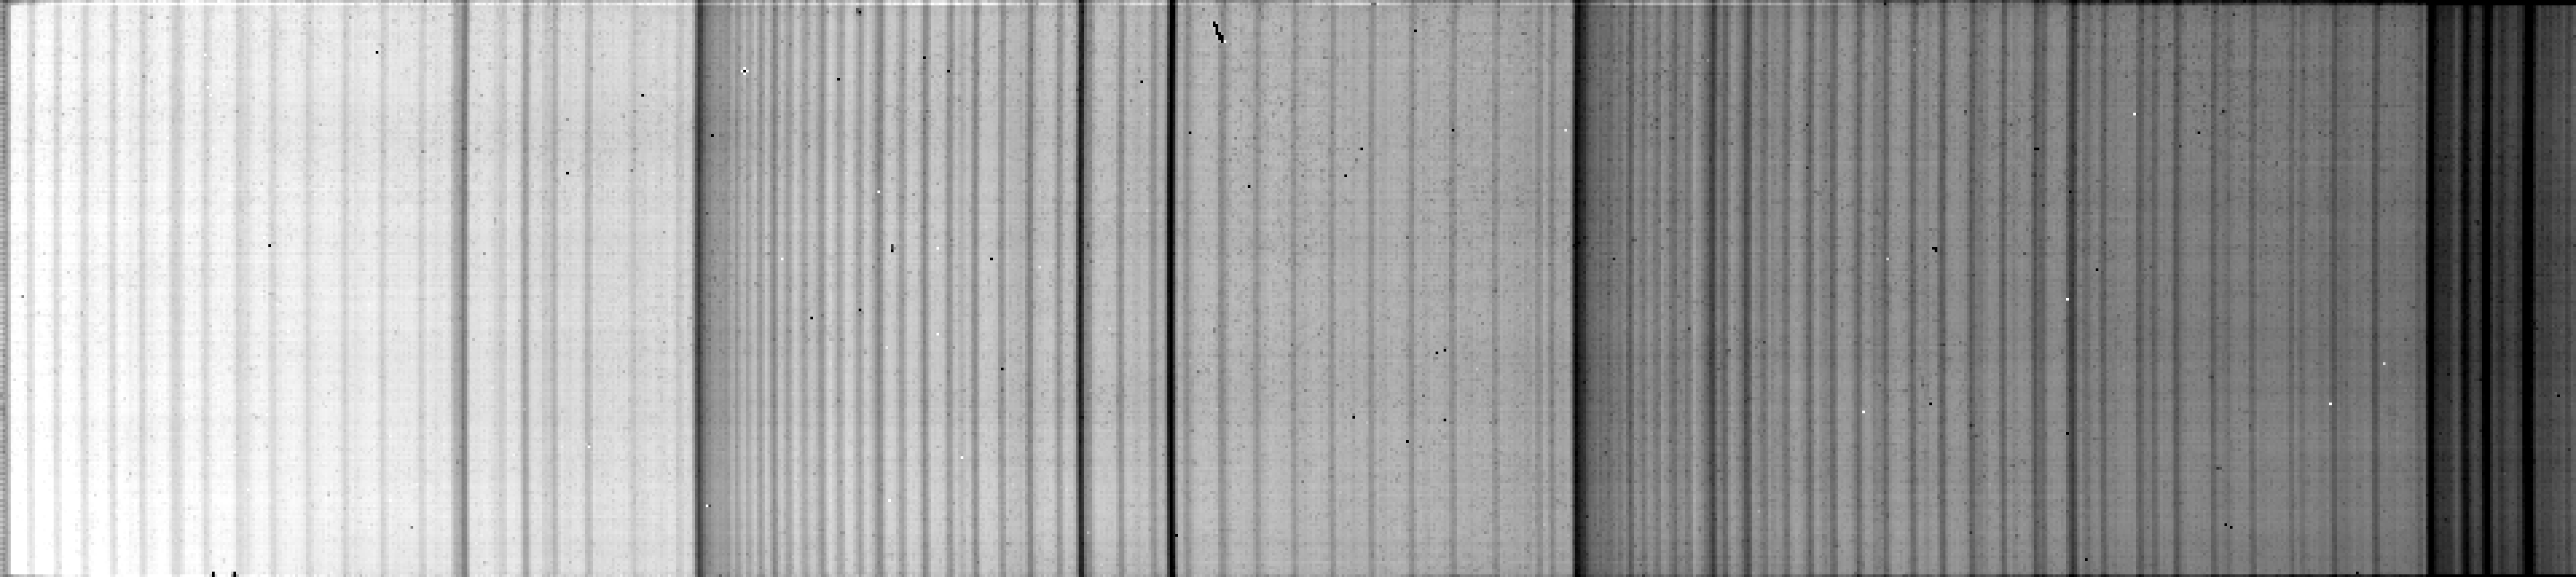
\includegraphics[width=\linewidth]{f/irradiance_78.png}\\
SWIR irradiance (bands 7 and 8)

Notice that there is a lot of data in the irradiance data.  In particular,
we see that the sun spectrum is not smooth (due to the absorption bands of
gases in the sun atmosphere).  Also, the individual pixel biases are very
visible in the irradiance images.

Thus the second method consists in simply computing the ratio
radiance/irradiance to obtain a top-of-the-atmosphere reflectance with less
artifacts.

\clearpage
The effect of computing this ratio for the averages of NIR bands is shown
below:

\begin{tabular}{ll}
	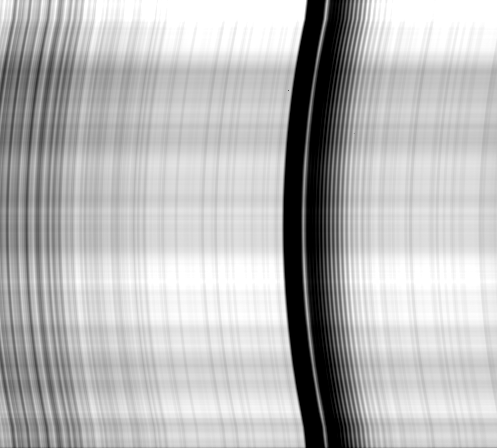
\includegraphics[width=0.48\linewidth]{f/b6_avgs_original.png} &
	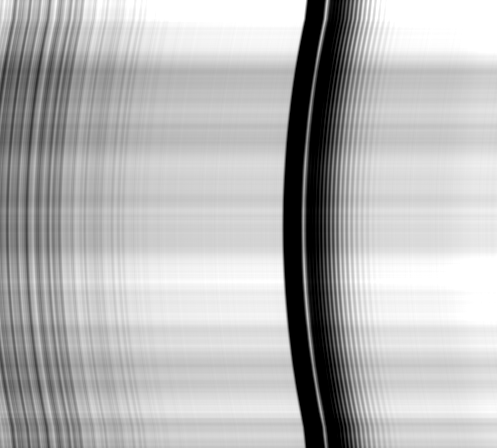
\includegraphics[width=0.48\linewidth]{f/b6_avgs_irradiance_corrected.png} \\
	$B6$ &
	$B6/IRRADIANCE$ \\
\end{tabular}

\begin{tabular}{ll}
	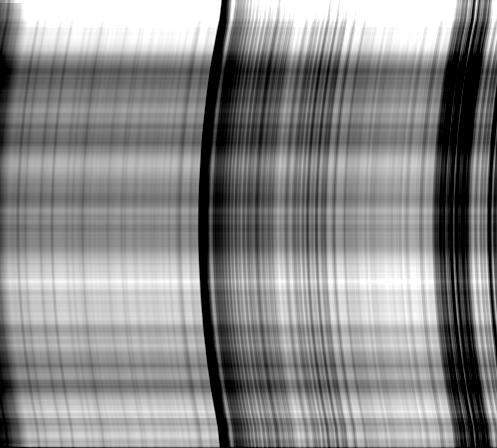
\includegraphics[width=0.48\linewidth]{f/b5_avgs_original.png} &
	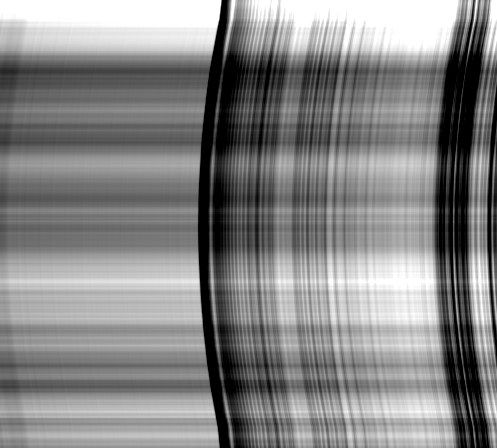
\includegraphics[width=0.48\linewidth]{f/b5_avgs_irradiance_corrected.png} \\
	$B5$ &
	$B5/IRRADIANCE$ \\
\end{tabular}

The effect of the ratio is striking: at some intervals of the spectrum,
there are no spectral lines in the sun nor in the earth atmospheres and we
see that the resulting ground albedo is very smooth (almost constant!).
Moreover all the bad pixels on these bands are correctly removed.

Unfortunately this is not the case for the SWIR band, where the bad pixels
evolve in a noticeable manner across one day, and this ratio does not remove
them completely.

\clearpage
\section{Comparison of both methods}

Advantages of the first method (data-based):

\begin{enumerate}
	\item the corrected image has still units of radiance
	\item only the bad pixels are corrected, the rest of the image is untouched
	\item the method needs only one image as input
	\item simple, conservative implementation; there's nothing to lose by
		applying this method
	\item transient pixels due to cosmic rays (which are per-image biases that
		decay very fast) can be corrected by this method
	\item can correct some unstable gains in SWIR that appear in only in one
		image
\end{enumerate}

Disadvantages of the data-based method:

\begin{enumerate}
	\item complex structured noise of the captor is not corrected, only
		individual bad pixels
	\item the method is simple but not trivial, some thresholds need to be set,
		etc.
\end{enumerate}


Advantages of the second method (irradiance-based):

\begin{enumerate}
	\item the method is trivial: just compute the ratio of two images
	\item all biases are corrected, not only isolated bad pixels
	\item the spectrum becomes much smoother, because we remove the spiky sun
		spectrum (see the graph below).  In other words, the dimensionality of
		the data is reduced.
	\item the corrected image is a relative reflectivity and takes values
		between 0 and 1 (often close to 1).
	\item visually more useful for bands UV, UVIS and NIR
\end{enumerate}

Disadvantages of the irradiance-based method:

\begin{enumerate}
	\item we need to download another file, and it is not clear which one: the
		irradiance acquired before or after the radiance image?
	\item the resulting image is unit-less
	\item inside the spectral holes of the sun light, this method enhances
		greatly the noise (the noise in the corrected image is not identically
		distributed)
	\item transient pixels cannot be corrected by this method, only long term
		biases of the sensor
	\item the SWIR sensor is very unstable and many bad pixels change between
		the irradiance and the radiance acquisitions.  Thus this method is not
		too useful for bands 7 and 8 (it leaves a fair amount of artifacts)
\end{enumerate}

The following graph shows the smoothing effect of dividing the radiance by
the irradiance (vertical scaling is arbitrary):

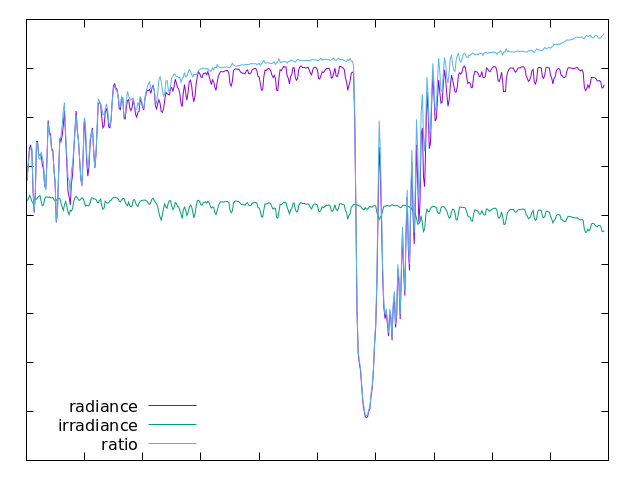
\includegraphics[width=\linewidth]{f/pixelratio.png}




\end{document}


% vim:set tw=77 filetype=tex spell spelllang=en ts=2 sw=2:
